\documentclass{article}
\usepackage[utf8]{inputenc}
\usepackage{hyperref}
\usepackage[letterpaper, portrait, margin=1in]{geometry}
\usepackage{enumitem}
\usepackage{amsmath}
\usepackage{booktabs}
\usepackage{graphicx}
\usepackage{amsmath}

\usepackage{hyperref}
\hypersetup{
colorlinks=true,
    linkcolor=black,
    filecolor=black,      
    urlcolor=blue,
    citecolor=black,
}
\usepackage{natbib}

\usepackage{titlesec}
\titleformat{\section}
{\normalfont\Large\bfseries}{\thesection}{1em}{}[{\titlerule[0.8pt]}]

\title{ECON7103 HW6}
\author{Sedat Ors}
\date{17 February 2023}

\begin{document}

\maketitle
\section{Python}
\vspace{0.5cm}
\begin{enumerate}

\item I think this is sharp RD. because the change in cutoff is dramatic and clear.

\item According to the graph in Figure 1 below, there seems discontinuity after and below cutoff.
\begin{figure}[]
    \centering
     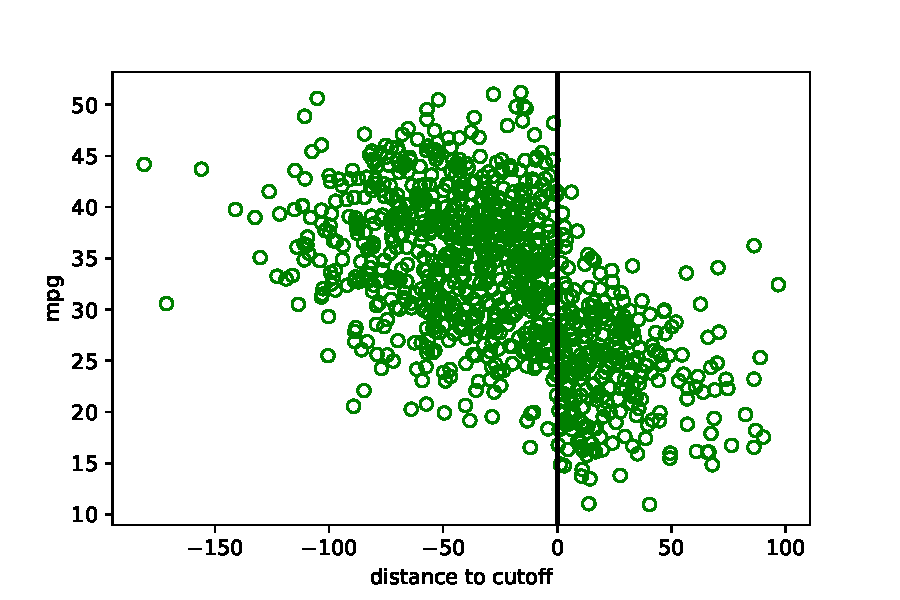
\includegraphics{HW6Q2.pdf}
    \caption{}
    \label{tab:question3}
\end{figure}

\item 
\begin{itemize}
    \item See Figure 2
    \item According to the result, the treatment leads reduction around 8.27 fuel efficiency per gallon at the cutoff. 
\end{itemize}

\begin{figure}[]
    \centering
     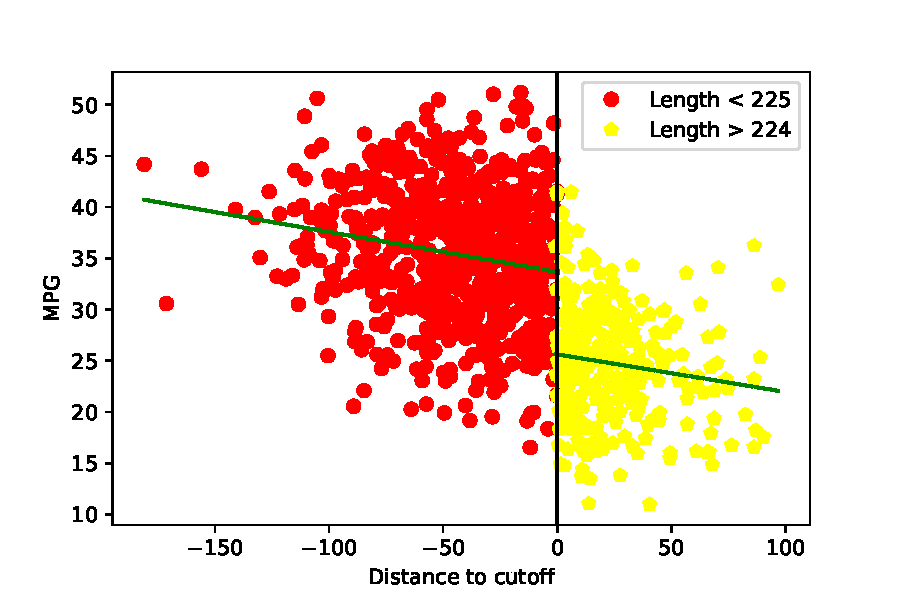
\includegraphics{HW6Q3a.pdf}
    \caption{}
    \label{tab:question3}
\end{figure}


\item 
\begin{itemize}
    \item See Figure 3
\item According to the result, at cut off, fuel efficiency is decreased by 8.05.
    
\end{itemize}

\item
 
\begin{figure}[]
    \centering
     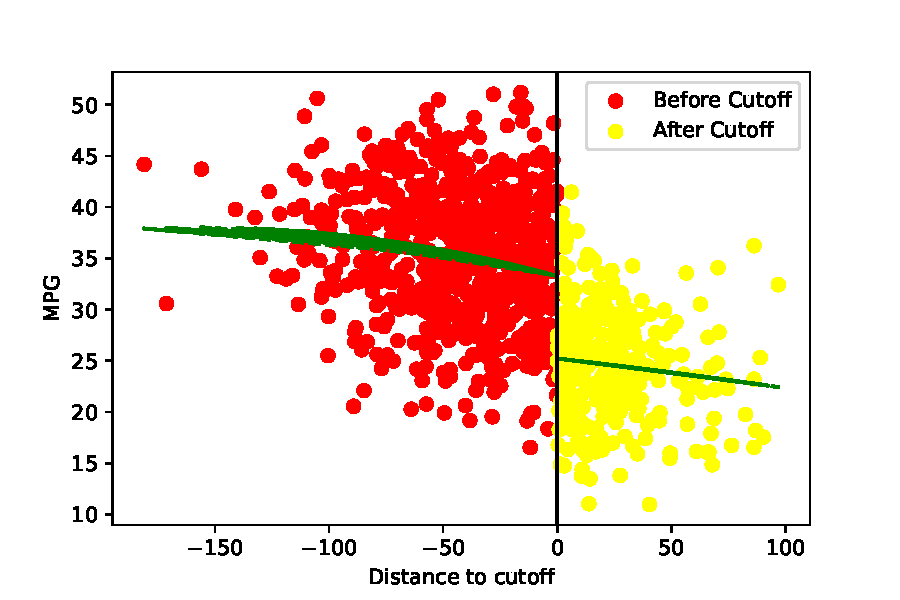
\includegraphics{HW6Q4a.pdf}
    \caption{}
    \label{tab:question3}
\end{figure}
\begin{itemize}
\item See Figure 4
\item Accordint to the result, at cut off, fuel efficiency is decreased by 7.44.

\end{itemize}
\begin{figure}[]
    \centering
     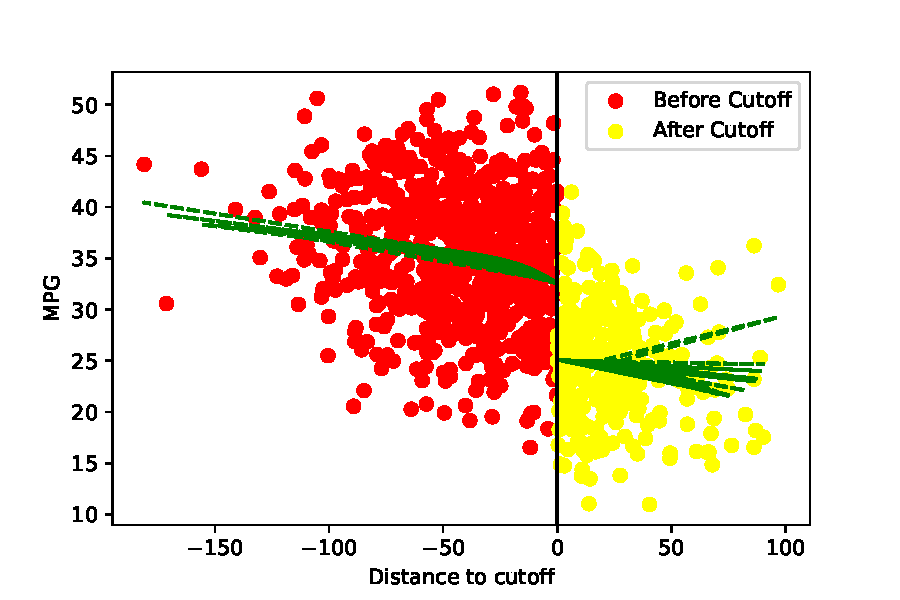
\includegraphics{HW6Q5a.pdf}
    \caption{}
    \label{tab:question3}
\end{figure}

\item According to the Table 1 below, the price is increases around 158\$, if level of mpg rise 1 unit.  
\vspace{0.5cm}
\begin{table}[]
    \centering
    \begin{tabular}{lc}
\toprule
{} &                    Q6 & Question 6 \\
\midrule
Sedan        &              -4747.32 &            \\
             &  (-5442.87, -4051.77) &            \\
MPG          &                158.78 &            \\
             &      (101.31, 216.24) &            \\
Constant     &              17392.94 &            \\
             &  (15741.11, 19044.78) &            \\
Observations &                       &       1000 \\
\bottomrule
\end{tabular}

    \caption{}
    \label{tab:question3}
\end{table}


    
\end{enumerate}
\section{Stata}

\begin{enumerate}

\item 
\begin{itemize}
    \item a) According to the figure 5(Table 2) below, the average treatment effect is 162\$. 
    \item b) See Figure 6
\end{itemize}

\begin{figure}[htbp]
\centering
\includegraphics[scale=0.9]{Table3.png}
\caption{Table 2}
\label{fig:}
\end{figure}

\begin{figure}[htbp]
\centering
\includegraphics[scale=0.4]{Table5.png}
\caption{}
\label{fig:}
\end{figure}

\vspace{0.5cm}
\item 

\vspace{0.5cm}

The IV should be correlated with the endogenous variable of interest. In other words, the IV should be able to explain some of the variations in the treatment variable and IV should not be correlated with the error term in the outcome equation.

I think mpg is statistically significant and according to the FSLS, the F value is bigger than 10. There is no endogeneity after 2SLS, we can say that this rd design is a good instrument.  
 

\end{enumerate}
\end{document}
